\documentclass[11pt]{article}

\usepackage{color}
%\input{rgb}
%----------Packages----------
\usepackage{amsmath}
\usepackage{amssymb}
\usepackage{amsthm}
\usepackage{amsrefs}
\usepackage{dsfont}
\usepackage{stmaryrd}
\usepackage{gensymb}
\usepackage{mathrsfs}
\usepackage{graphicx, nicefrac}
\usepackage[colorlinks=true,linkcolor=blue]{hyperref}
\usepackage[mathcal]{eucal}
\usepackage{verbatim}  %%includes comment environment
\usepackage{fullpage}  %%less massive margins
\usepackage{graphicx}
\usepackage{siunitx}
\usepackage[english]{babel}
\usepackage[square,numbers]{natbib}
\usepackage{float}
\usepackage{caption}
\usepackage{cancel}
\usepackage{braket}
\usepackage{mathtools}
\usepackage{physics}
\usepackage{empheq}
\usepackage{bbm}
\usepackage[most]{tcolorbox}
\usepackage{booktabs} % For prettier tables
\hypersetup{colorlinks=true, linkcolor=blue, urlcolor=blue, citecolor=blue}
\bibliographystyle{abbrvnat}
\captionsetup{labelfont=bf}
\graphicspath{ {./images/} }
%----------Commands----------

%%penalizes orphans
\clubpenalty=9999
\widowpenalty=9999

%% shortcuts because im lazy
\newcommand{\eps}{\epsilon}
\newcommand{\veps}{\varepsilon}
\newcommand{\sig}{\sigma}
\newcommand{\nfrac}{\nicefrac}
\newcommand{\lam}{\lambda}
\newcommand{\gam}{\gamma}
\newcommand{\kap}{\kappa}
\newcommand{\del}{\nabla}
\newcommand{\Del}{\Delta}
\newcommand{\tht}{\theta}
\newcommand{\east}{^\ast}
\newcommand{\non}{\nonumber}
\newcommand{\om}{\omega}
\newcommand{\alp}{\alpha}
\newcommand{\bbR}{\mathbb{R}}
\newcommand{\bbC}{\mathbb{C}}
\newcommand{\bbP}{\mathbb{P}}
\newcommand{\bbZ}{\mathbb{Z}}
\newcommand{\bbN}{\mathbb{N}}
\newcommand{\cC}{\mathcal{C}}
\newcommand{\cB}{\mathcal{B}}
\newcommand{\cL}{\mathcal{L}}
\newcommand{\bS}{\mathbf{S}}
\newcommand{\bB}{\mathbf{B}}
\newcommand{\bE}{\mathbf{E}}
\newcommand{\bn}{\mathbf{n}}
\newcommand{\bx}{\mathbf{x}}
\newcommand{\br}{\mathbf{r}}
\newcommand{\bq}{\mathbf{q}}
\newcommand{\bk}{\mathbf{k}}
\newcommand{\bA}{\mathbf{A}}
\newcommand{\bP}{\mathbf{P}}
\newcommand{\bH}{\mathbf{H}}
\newcommand{\bD}{\mathbf{D}}
\newcommand{\bj}{\mathbf{j}}
\newcommand{\ba}{\mathbf{a}}
\newcommand{\cE}{\mathcal{E}}
\newcommand{\vv}{\vec{v}}
\newcommand{\nhat}{\hat{n}}
\newcommand{\xhat}{\hat{x}}
\newcommand{\yhat}{\hat{y}}
\newcommand{\zhat}{\hat{z}}
\newcommand{\vx}{\vec{x}}
\newcommand{\proj}{\mrm{Proj}}
\newcommand{\Ryd}{\rm{Ryd}}
\renewcommand{\_}[1]{\underline{ #1 }}
\newcommand{\fmag}[1]{\left\lVert #1 \right\rVert}
\newcommand{\oline}{\overline}
\newcommand{\wt}{\widetilde}
\newcommand{\mrm}{\mathrm}
\newcommand{\lpc}{\vec{\nabla}^2}
\newcommand{\fdele}{\pdv{x}+\pdv{y}+\pdv{z}}
\newcommand{\fdelte}{\pdv[2]{x}+\pdv[2]{y}+\pdv[2]{z}}
\newcommand{\Gam}{\Gamma}
\renewcommand{\l}{\ell}
\newcommand{\lm}{\ell\ m}
\newcommand{\sint}{\sin\theta}
\newcommand{\cost}{\cos\theta}
\newcommand{\sinp}{\sin\phi}
\newcommand{\cosp}{\cos\phi}
\newcommand{\im}{\mathrm{im}}
\newcommand{\balls}{\bigcirc\bigcirc}
\newcommand{\dagg}{^\dagger}
\newcommand{\orth}{^{\perp}}
\newcommand{\conj}{^\ast}
\renewcommand{\deg}{^{\circ}}
\newcommand{\braketmatrix}[3]{\left \langle #1 \middle| #2 \middle| #3 \right \rangle}
\newcommand{\infint}{\int_{-\infty}^{\infty}}
\newcommand{\infiiint}{\infint\infint\infint}
\newcommand{\sqmod}[1]{\abs{ #1 }^2}
\newcommand{\sh}{Y_{\l}^m}
\newcommand{\sharg}{Y_{\l}^m(\theta,\phi)}
\newcommand{\rtp}{(r,\theta,\phi)}
\newcommand{\tp}{(\theta,\phi)}
\newcommand{\npar}{\vspace{.3cm}\newline}
\newcommand{\nparii}{\npar\indent}
\newcommand{\un}{~\rm}
\newcommand{\boltzmann}{1.381 \cdot 10^{-23} \un{J/K}}
\newcommand{\gravconstant}{6.67 \cdot 10^{-11} \un{N m^2/kg^2}}
\newcommand{\Msun}{1.989 \cdot 10^{30} \un{kg}}
\newcommand{\Rsun}{6.957 \cdot 10^8 \un{m}}
\newcommand{\mH}{1.673 \cdot 10^{-27} \un{kg}}
\newcommand{\planck}{6.626 \cdot 10^{-27} \un{(g\cdot cm^2)/s}}
\newcommand{\speedoflight}{2.998\cdot 10^{10} \un{cm/s}}
\newcommand{\stephboltzmann}{5.670 \cdot 10^{-5} \un{g/(s^3 \cdot K^4)}}
\renewcommand{\cross}{\times}
\newcommand{\sun}{_{\odot}}
\newcommand{\eff}{_{\rm{eff}}}
\newcommand{\us}{\textunderscore}
\newcommand*\widefbox[1]{\fbox{\hspace{.25em}#1\hspace{.25em}}}

%\renewcommand{\phi}{\varphi}

\renewcommand{\emptyset}{\O}

\providecommand{\abs}[1]{\lvert #1 \rvert}
\providecommand{\norm}[1]{\lVert #1 \rVert}


\providecommand{\ar}{\rightarrow}
\providecommand{\arr}{\longrightarrow}

\DeclareMathOperator{\ext}{ext}

%\begin{bmatrix}[ccc|c] STUFF \end{bmatrix}
\makeatletter
\renewcommand*\env@matrix[1][*\c@MaxMatrixCols c]{%
  \hskip -\arraycolsep
  \let\@ifnextchar\new@ifnextchar
  \array{#1}}
\makeatother

\newcommand{\head}[1]{
	\begin{center}
		{\large #1}
		\vspace{.2 in}
	\end{center}
}

\newcommand{\fdel}[1] {
	\pdv{#1}{x}+\pdv{#1}{y}+\pdv{#1}{z}
}

\newcommand{\fdelt}[1]{
	\pdv[2]{#1}{x}+\pdv[2]{#1}{y}+\pdv[2]{#1}{z}
}

\newcommand{\infsum}[1]{
	\sum_{#1=0}^{\infty}
}

\newcommand{\sub}[1]{
    _{\rm{#1}}
}

%----------Title-------------


\begin{document}

\head
{Ariel Barnea\\June 2023\\Argonne National Laboratory\\Final Bispectrum Report}

\vspace{-1cm}
\hypersetup{linkcolor=black}
\renewcommand\contentsname{Table of Contents}
\tableofcontents
\newpage

\hypersetup{linkcolor=blue}

{\setlength{\parindent}{0cm}

\section{Introduction}\label{intro}

\subsection{What is the Bispectrum}

The Power Spectrum has long served as a reliable tool for analyzing the statistical properties of cosmic structures. In a Gaussian universe, it summarizes all of the essential information necessary to characterize the distribution of power across different angular scales. However, in our real universe, additional complexities arise, driven by gravitationally-induced non-Gaussianity. To extract a more comprehensive understanding of the underlying physics encoded in cosmological maps, we must turn to the Bispectrum.
\npar
The Bispectrum is a higher-order statistical measure that, by examining the correlations among three different angular modes, allows us to unravel non-Gaussian signatures that the Power Spectrum cannot. When seeking to understand the primordial universe and the formation and evolution of cosmic structures, understanding the presence of non-Gaussianities is crucial. Furthermore, the Bispectrum's unique property of incorporating three factors, compared to the two factors found in the power spectrum, provides an opportunity to break degeneracies that might be present in the latter. By scrutinizing the Bispectrum's additional degree of freedom, we can disentangle these degeneracies and gain a deeper understanding of the underlying physical phenomena.
\npar
As such, by exploring the Bispectrum, and specifically doing so in harmonic space, we can seek to understand a small subsegment of the the complexities of our universe, and hopefully learn a bit on how cosmic evolution operated.

\subsection{The Purpose of this Report}

I am writing this report to serve as a guide for any future researchers interested in the Bispectrum and non-Gaussianities. It is intended to explain all of the code I have written and the plots I have created during my time working on the Bispectrum project at Argonne National Laboratory. I also seek to explain the methodology and process behind the work of this project, so that any future researchers won't fall into some of the issues that we ran into and had to troubleshoot and fix. This guide also seeks to compile much of the theory, equations, and papers that underly the Power Spectrum and gravitationally-induced weak-lensing Bispectrum into one big guide that is readily accessible. Hopefully, this will also allow for a more bite-sized approach to understanding the maths behind the Bispectrum, as my goal is to compile this information in a more readable way. Finally, this guide also serves as a place to discuss some of the computational methods that I have learned in my time at Argonne. I seek to do so in a way that will help future researchers not have to go searching through the depths of Python package documentations and YouTube tutorials like I had to, and instead be a personal guide to understanding the underlying infrastructure and applications of these computational methods. I conclude this report with a brief discussion on the possible directions for future research with this project and Bispectrum code, along with some thoughts on what I learned from this project and my time working for the Computational Physics and Advanced Computing Group at Argonne National Laboratory, and a final acknowledgements (i.e. thank you's) to people that helped me along the way.

\section{Methodology and Process}\label{methodology}

In this section, I discuss the theory behind the two main methods that we utilized when creating the Bispectrum calculator. This is in Section~\ref{theory}. Then, in Sections~\ref{wigner} and ~\ref{numba}, I go into some of the challenges that we ran into and the lessons we learned from trying to speed up the code from its prototype version.

\subsection{Theory Calculations and Equations}\label{theory}

This subsection is intended to give an overview / compile all of the different theory calculations, equations, and information that others might find useful to have all in one place, if you are trying to delve into the world of Bispectrum calculations.

\subsubsection{Filter Average Method}\label{averagemethod}

The first method I will go into is the filter method, pulled from \cite{Bucher_2016}, which seeks to estimate the value of the bispectrum (and later, binned bispectrum). This method is primarily focused on calculating the individual $B_{\ell_1 \ell_2 \ell_3}$ values of the bispectrum and averaging them to find the overall averaged bispectrum. The equation for doing this is:
\begin{equation}
    B_{\ell_1\ell_2\ell_3} = \sqrt{N_{\Delta}^{\ell_1\ell_2\ell_3}} \sum_{m_1,m_2,m_3}
    \begin{pmatrix}
        \ell_1 & \ell_2 & \ell_3 \\
        m_1 & m_2 & m_3
    \end{pmatrix}
    \langle a_{\ell_1 m_1} a_{\ell_2 m_2} a_{\ell_3 m_3} \rangle
\end{equation}

where the normalization factor is given by:

\begin{equation}
N_{\Delta}^{\ell_1\ell_2\ell_3} = \frac{(2\ell_1+1)(2\ell_2+1)(2\ell_3+1)}{4\pi}
    \begin{pmatrix}
        \ell_1 & \ell_2 & \ell_3 \\
        0 & 0 & 0
    \end{pmatrix}^2
\end{equation}

Here, the quantity $\langle a_{\ell_1 m_1} a_{\ell_2 m_2} a_{\ell_3 m_3} \rangle$ is the CMB angular bispectrum and $N_{\Delta}^{\ell_1 \ell_2 \ell_3}$ can be thought of as the number of possible $(\ell_1, \ell_2, \ell_3)$ triangles on the celestial sphere. Note the use of the Wigner-3j values (see Section~\ref{wigner}) here. Also note that we excluded the polarization factors because we're dealing with scalar temperature fields. Further important information to note about these equations include that:
\begin{enumerate}
    \item The bispectrum is symmetric under the simultaneous exchange of its three multiple numbers $\ell_1$, $\ell_2$, $\ell_3$. Basically, we can just restrict our computation of $B_{\ell_1 \ell_2 \ell_3}$ to $\ell$ values s.t. $\ell_1 \leq \ell_2 \leq \ell_3$.
    \item The triangular condition must be satisfied, i.e. $\ell_1 + \ell_2 + \ell_3 = \text{constant}$.
    \item The parity condition must be satisfied, i.e. $\ell_1 + \ell_2 + \ell_3 = \text{even}$.
    \item The triangle inequality is satisfied, i.e. $\abs{\ell_1 - \ell_2} \leq \ell_3 \leq \ell_1 + \ell_2$.
\end{enumerate}

Conditions 3 and 4 come from the fact that the $m$ values in the normalization factor are all equal to $0$. These conditions are very useful, and I would recommend becoming familiar with them as they speed up maths and computations.
\npar
We also went into the theoretical variance for this calculation, which is given by:

\begin{equation}
    \operatorname{Var}\left(B_{\ell_{1} \ell_{2} \ell_{3}}\right)=g_{\ell_{1} \ell_{2} \ell_{3}} N_{\Delta}^{\ell_{1} \ell_{2} \ell_{3}} C_{\ell_{1}} C_{\ell_{2}} C_{\ell_{3}} \equiv V_{\ell_{1} \ell_{2} \ell_{3}}
\end{equation}

such that $N_{\Delta}^{\ell_1 \ell_2 \ell_3}$ is as before, namely:
\begin{equation}
    N_{\Delta}^{\ell_1\ell_2\ell_3} = \frac{(2\ell_1+1)(2\ell_2+1)(2\ell_3+1)}{4\pi} \begin{pmatrix}
        \ell_1 & \ell_2 & \ell_3 \\
        0 & 0 & 0
    \end{pmatrix}^2
\end{equation}

and $g_{\ell_1 \ell_2 \ell_3}$ is equal to either 6, 2, or 1 depending on whether 3, 2, or no $\ell$'s are equal respectively. This implies that, for the equilateral case we're dealing with above, $g_{\ell_1 \ell_2 \ell_3} = 6$, giving us a variance:

\begin{equation}
    V_{\ell_1 \ell_2 \ell_3} = 6 \cdot N_{\Delta}^{\ell_1 \ell_2 \ell_3} \cdot C_{\ell_1} C_{\ell_2} C_{\ell_3}
\end{equation}

It should be noted that, for the binned bispectrum:
\begin{equation}
    B_{i_1 i_2 i_3} = (\Xi_{i_1 i_2 i_3})^{-1} \sum_{\ell_1\in\Delta_1}\sum_{\ell_2\in\Delta_2}\sum_{\ell_3\in\Delta_3} B_{\ell_1 \ell_2 \ell_3}
\end{equation}

where $\Xi_{i_1 i_2 i_3}$ is the number of $\ell$ triplets within the $(i_1,i_2,i_3)$ bin triplet satisfying the triangle inequality and parity condition selection rule, the variance $\operatorname{Var} (B_{i_1 i_2 i_3})$ is:

\begin{equation}
    \operatorname{Var} (B_{i_1 i_2 i_3}) = \frac{g_{i_1 i_2 i_3}}{(\Xi_{i_1 i_2 i_3})^2} \sum_{\ell_1\in\Delta_1}\sum_{\ell_2\in\Delta_2}\sum_{\ell_3\in\Delta_3} N_{\Delta}^{\ell_1 \ell_2 \ell_3} C_{\ell_1} C_{\ell_2} C_{\ell_3} \equiv V_{i_1 i_2 i_3}
\end{equation}


\subsubsection{Map Method}\label{mapmethod}

The second method I will go into is the map method, also pulled from \cite{Bucher_2016}. This also seeks to estimate the value of the bispectrum, but utilizes a map-based approach instead of a computation, filter averaged method.
\npar
This method stems from the straightforward computation of evaluating the integral over the sky:
\begin{equation}
    B_{\ell_1 \ell_2 \ell_3}^{p_1 p_2 p_3, \rm{obs}} = \int \dd{\hat{\Omega}} M_{\ell_1}^{p_1, \rm{obs}}(\hat{\Omega}) M_{\ell_2}^{p_2, \rm{obs}}(\hat{\Omega}) M_{\ell_3}^{p_3, \rm{obs}}(\hat{\Omega})
\end{equation}

where the $\ell$ triplets here also satisfy the selection rules from the Filter Method. This computation would take a lot of time if not for the fact that binning leads to a massive reduction in computational cost with minimal resolution loss. To accomplish this, we divide the $\ell$-range $\left[\ell_{\min }, \ell_{\max }\right]$ into subintervals denoted by $\Delta_i=\left[\ell_i, \ell_{i+1}-1\right]$ where $i=0, \ldots,\left(N_{\text {bins }}-1\right)$ and $\ell_{N_{\text {bins }}}=\ell_{\max }+1$, so that the filtered maps are:
\begin{equation}
M_i^p(\Omega)=\sum_{\ell \in \Delta_i} \sum_{m=-\ell}^{+\ell} a_{\ell m}^p Y_{\ell m}(\hat{\Omega})
\end{equation}

and we use these instead of $M_{\ell}^p$ in our expression for $B_{\ell_1 \ell_2 \ell_3}^{p_1 p_2 p_3, \rm{obs}}$. The binned bispectrum is thus:
\begin{equation}
    B_{i_1 i_2 i_3}^{p_1 p_2 p_3, \mathrm{obs}}=\frac{1}{\Xi_{i_1 i_2 i_3}} \int d \hat{\Omega} M_{i_1}^{p_1, \mathrm{obs}}(\hat{\Omega}) M_{i_2}^{p_2, \mathrm{obs}}(\hat{\Omega}) M_{i_3}^{p_3, \mathrm{obs}}(\hat{\Omega})
\end{equation}

where $\Xi_{i_1 i_2 i_3}$ is the number of $\ell$ triplets within the $\left(i_1, i_2, i_3\right)$ bin triplet satisfying the triangle inequality and parity condition selection rule. The authors of this paper explain that $B_{i_1 i_2 i_3}^{p_1 p_2 p_3}$ can thus be thought of as an average over all valid $B_{\ell_1 \ell_2 \ell_3}^{p_1 p_2 p_3}$ in the bin triplet.
\npar
This method allows for a relatively straightforward and quick computation of $B_{i_1 i_2 i_3}$ from $a_{\ell m}$, as we will see in Section~\ref{code}.

\subsubsection{Convergence Bispectrum}\label{convergencebispec}

Most recently, we worked on finding the theoretical convergence bispectrum found in \cite{Munshi_2020}:
\begin{equation}
    B_{\ell_1, \ell_2, \ell_3} = \int_0^{\chi_s} d\chi \left[\frac{3\Omega_M H_0^2}{2a(\chi)}\right]^3 \chi^2 W^3(\chi, \chi_s) B_{\delta}\left(\frac{\ell_1}{\chi}, \frac{\ell_2}{\chi}, \frac{\ell_3}{\chi}, \chi\right)
\end{equation}

such that:
\begin{equation}
    k_i = \frac{\ell_i}{\chi}
\end{equation}

where $B_{\delta}(\mathbf{k}_1, \mathbf{k}_2, \mathbf{k}_3; \chi)$ is given by:
\begin{equation}
    B_{\delta}(\mathbf{k}_1, \mathbf{k}_2, \mathbf{k}_3; \chi) = 2F_2(\mathbf{k}_1, \mathbf{k}_2, z)P_{\delta}(\mathbf{k}_1,z)P_{\delta}(\mathbf{k_2},z) + \text{cyc. perm}
\end{equation}

and
\begin{equation}
    F_2(\mathbf{k}_1, \mathbf{k}_2, z) = \frac57 a(k_1, z)a(k_2, z) + \frac12 \frac{k_1^2 + k_2^2}{k_1k_2}b(k_1, z)b (k_2,z)\cos\theta + \frac27 c(k_1, z)c(k_2,z)
\end{equation}

where we're using $a = b = c = 1$, giving us:

\begin{equation}
    F_2(\mathbf{k}_1, \mathbf{k}_2, z) = \frac57 + \frac12 \frac{k_1^2 + k_2^2}{k_1k_2}\cos\theta + \frac27
\end{equation}

Which is needed for every cyclical permutation. We also require the lensing kernel $W(\chi, \chi_s)$, which is given by:
\begin{equation}
    W(\chi, \chi_s) = \frac{\chi_s - \chi}{\chi\chi_s}\Theta(\chi_s - \chi)
\end{equation}

where the step function $\Theta(\chi_s - \chi)$ is there to ensure that the lensing can’t have a contribution from before the source existed. We can control this via integration, so we'll let $\Theta(\chi_s - \chi) = 1$, leaving us with:

\begin{equation}
    W(\chi, \chi_s) = \frac{\chi_s - \chi}{\chi\chi_s}
\end{equation}

Note that, for the CMB, the redshift is just $z = 1089$. Implementing all of this together yields the convergence bispectrum for a set of $\ell_1$, $\ell_2$, $\ell_3$ values, and can be done for $\ell$-bins to find the binned convergence bispectrum for some map.

\subsubsection{Bispectrum Templates}

A brief tangent I went down whilst writing my initial bispectrum function is the different local vs. non-local bispectrum templates. More information about these Bispectrum templates and non-Gaussianities overall can be found in \cite{Woods_2018}, which was instrumental in helping me understand these topics. For local $f_{\rm NL}$ potential, we have:
\begin{equation}
    \phi_{\rm NL} = \phi_{\rm Gauss} + f_{\rm NL} \left(\phi_{\rm Gauss}^2 - \langle\phi_{\rm Gauss}\rangle^2\right)
\end{equation}

For $g_{\rm NL}$, we have:
\begin{equation}
    \phi_{\rm NL} = \phi_{\rm Gauss} + g_{\rm NL}\left(\phi_{\rm Gauss}^3\right)
\end{equation}

And for non-local $f_{\rm NL}$, we have:
\begin{equation}
    \phi_{\rm NL} = \phi_{\rm Gauss} + f_{\rm NL}\left(\partial\phi_{\rm Gauss}^2 - \langle \partial \phi_{\rm Gauss} \rangle^2 \right)
\end{equation}

\subsubsection{Some Power Spectrum Notes}\label{powerspecnotes}

As a brief aside, I will discuss later some of the code I wrote for computing and plotting Power Spectra, so I will use this short section to detail the finite and infinite spherical shell cases for computing the Power Spectrum. More information about these cases can be found in \cite{Takahashi_2017}.
\npar
The equation for finding $C_{\ell}$ from $P(k)$ assuming we're $\textit{not}$ dealing with a finite spherical thin shell is given by:
\begin{equation}
    C_{\ell} = \frac{2}{\pi}\int_0^{\infty} dk\cdot k^2\cdot P(k)\cdot \left|\frac{\Theta_{\ell}(k)}{\delta(k)} \right|^2
\end{equation}

However, noting that the plots we usually work with are already overdensity plots, implying that $\Theta_{\ell}(k)=\delta(k)$, we find:
\begin{equation}
    \left| \frac{\Theta_{\ell}(k)}{\delta(k)}\right|^2 = \left|\frac{\delta(k)}{\delta(k)}\right|^2 = 1
\end{equation}

Therefore, for the ideal case, we find:
\begin{equation}
    C_{\ell} = \frac{2}{\pi}\int_0^{\infty} dk\cdot k^2\cdot P(k)
\end{equation}

Now, when we're dealing with a finite spherical thin shell, we have to amend our previous equation with a $\texttt{sinc}$ correction factor. This, we find a $C_{\ell}$ expression for the finite case of:
\begin{equation}
    C_{\ell}^{\text{shell}} = \frac1{r^2} \int \frac{dk_{\parallel}}{2\pi}\cdot P_{\delta}(k)\cdot \rm{sinc}\left(\frac{k_{\parallel}\Delta r}{2}\right)
\end{equation}

such that $k = (k_{\parallel}^2 + |\mathbf{k}_{\perp}|^2)^{1/2}$, where $\mathbf{k}_{\perp} = \ell/r$. However, in the case of the infinite shell, we can just take the limit as $k_{\parallel}\Delta r\to\infty$ of the thin spherical shell, which would give us:
\begin{equation}
    \lim_{k_{\parallel}\delta r\to\infty} C_{\ell}^{\text{shell}} = \frac{1}{r^2\Delta r} P_{\delta}\left(k=\frac{\ell}{r}\right)
\end{equation}

\subsection{Numba}\label{numba}

Numba is a Just-In-Time (JIT) compiler for Python that specializes in optimizing and accelerating numerical computations. If you are a Python-only coder like I was when I first started using Numba and don't understand what this means, don't worry, I will explain it here! I will also explain how to use Numba, and why you should use Numba for computationally expensive and \textit{repetitive} tasks that don't involve sharing memory allocation.
\npar
First, a brief explanation of why we use Numba. Python is a very convenient, simple, and easy-to-use language with a lot of capabilities. You don't have to declare types, worry about pointers, allocate and free memory, etc. However, to allow the users (us) to get away with all of this, Python has to do all of this stuff internally. For example, declaring $i = 0$, you don't have to state that $i$ is an integer or unsigned integer, as Python will do this for you by creating an integer object with a value of $0$ and a ``reference'' $i$. But to access $i$, you have to access an object, not just straight bytes (i.e. a bunch of $0$ and $1$ bits). Creating and appending to lists means that Python has to allocate a bunch of space for the list, way more than you will probably need, and then tie the values in your list together every time you append. So basically, this makes things very convenient for you as the user, but not very computationally efficient, as it has to go through the Python interpreter and deal with all of this convenience.\footnote{This is why C is extremely speedy, because it compiles straight down into assembly and then machine code, and doesn't have to go through all of these hoops to operate | but it requires a lot more strict control, typesetting, and memory management.}
\npar
Numba bridges this gap with Python by compiling your Python code straight into highly-efficient machine code using just-in-time compilation techniques. Using the \texttt{@jit} function decorator (I will explain this shortly) on a function allows Numba to analyze the function code and apply various optimizations. It inspects the types of the input arguments and generates optimized machine code specific to those types. This process is known as type specialization. \texttt{@njit} is another Numba function decorator which stands for \texttt{No Python jit}, which is basically just ``jitting'' a function but without going through the Python interpreter. It is very important to note that jitting a function means you lose a lot of Python's capabilities (i.e. calling complex functions that aren't also jit-compatible, using Python data structures like lists and dictionaries, etc.). That's why jitting is so useful for repetitive computations like loops, where C shines, but not used for things like plotting, where Python shines. Since computing the Bispectrum, specifically the filter average method from Section~\ref{averagemethod}, requires a lot of looping and summing and not many Pythonic data structures and functions, this makes our Bispectra calculations a prime candidate for Numba. Hence why this section exists. However, before I get into how I used Numba, I want to talk briefly about parallelization.
\npar
Another very useful element of Numba is that you can parallelize your code across multiple threads. I primarily used the parallel loops functionality of Numba, as most of my Bispectrum calculations involved two or three nested for loops at a time (for example, when summing over all of the $m$ values in an $\ell_1$ and $\ell_2$ range, or summing over all of the $\ell$-values in an $i$-bin). Basically what this means is that I split up my computation of $B_{\ell_1 \ell_2 \ell_3}$ across multiple \textit{threads}. Threads are basically just independently run portions of a program that can be spread across multiple cores of your computer and run simultaneously. When you launch $n$ threads, you can think of your computer distributing the function into $n$ different parts and running them all concurrently. For example, if you want to thread a function that sums all the values from $1$ to $1600$ across $16$ threads, you can distribute the summing of the values $1$ to $100$ to thread 1, values $101$ to $200$ to thread 2, $201$ to $300$ to thread 3, etc.\footnote{This is not a good way to distribute this computation by the way, I'm just using this as an example.} This is a very useful concept in Computer Science, but not one I am going to flesh out today. Instead, I am going to talk about Numba's \texttt{parallel=True} capabilities when in a jitted function. Activating this flag will basically let Numba know that you want to distribute the function's job across multiple threads, and it will do it automatically across the number of threads you provide (normally, you have to manually do this). This automatic threading only works for \textit{loops} (since it's simple enough without having to do it manually), but conveniently, that's exactly what we need it for. So, when summing up Bispectrum values\footnote{Notice that this does not involve storing any values anywhere, which is why this works.}, you can parallelize the for loops across $n$ threads to speed up your computation by \textit{about} $n$ times.\footnote{Overhead costs of initializaing your threads and passing in the necessary parameters can slow this down.}
\npar
Okay, now I will very briefly explain how to use Numbas capabilities. Basically, whenever you want to jit a function, first make sure it can be jitted (otherwise Numba will give you an error), which you can do by checking if you have any non-jitted function calls or are using a bunch Pythonic data types in your function like dictionaries, lists, and/or objects. Then, you just add the jit function decorator \texttt{@njit} to the line before the function declaration, like:
\begin{verbatim}
    @njit
    def foo(x: int) -> int:
        return x
\end{verbatim}

And that's it, your function is now jitted in no Python mode. To parallelize a loop specifically, you can just add the flag \texttt{parallel=True} to your function decorator, and then use a function like \texttt{prange} on a loop instead of \texttt{range}. For example:
\begin{verbatim}
    @njit(parallel=True)
    def bar(n: int) -> int:
        sum = 0
        for i in prange(n):
            sum += i
        return sum
\end{verbatim}

\texttt{prange} basically just distributes the job of looping across multiple threads. If you want to set the number of threads, you can just include the function \texttt{set\textunderscore num\textunderscore threads(n\textunderscore threads)}, where \texttt{n\textunderscore threads} is some integer number of threads, somewhere in the function, and that's it! For example:
\begin{verbatim}
    @njit(parallel=True)
    def bar(n: int, num_threads: int) -> int:
        sum = 0
        set_num_threads(n_threads)
        for i in prange(n):
            sum += i
        return sum
\end{verbatim}

And don't forget to import all of these functions, by the way.
\begin{verbatim}
    from numba import jit, njit, prange, set_num_threads
\end{verbatim}

Congratulations, that's basically everything you need to know about Numba for the purposes of Bispectrum computations!
%
\npar
\textbf{An Aside: Numba Typing}
\npar
If you want to used lists and dictionaries with jitted functions, look into Numba's Typed libraries to declare these Numba-specific types. Basically, it just declares a specific type for the entire data structure so that Numba can parse it. You can find more information in Numba's documentation.

\subsection{Wigner-3j}\label{wigner}

The Wigner-3j coefficients play a big role in many Bispectrum computations, so I am using this section to briefly discuss how we used them, the (many) issues we encountered with them, and how you can hopefully not have to deal with these because of this guide!
\npar
There were two main packages we used to compute the Wigner-3j coefficients, each with their benefits and drawbacks. I will summarize them both and explain which one we ended up using.

\subsubsection{Spherical Wigner-3j Calculator}

The first Python package I used to compute the Wigner-3j coefficients was \texttt{spherical}.\footnote{\href{https://pypi.org/project/spherical/}{https://pypi.org/project/spherical/}.} Spherical is specifically designed for evaluating and transforming Wigner's $\mathcal{D}$ matrices, Wigner's 3-j symbols, and spin-weighted (and scalar) spherical harmonics. I believe it relies on a recursive equation set to calculate the w3j values, and it does so very quickly. It also works in combination with numba's just-in-time environment, which is extremely useful for the filter average method of computing the Bispectrum, as explained in Section~\ref{averagemethod}.
\npar
This was my package of choice at the start. However, this package has two glaring issues that proved fatal.

\begin{enumerate}
    \item \textbf{It can't compute Wigner-3j values for high $\ell$, which I found to be somewhere around $\ell \approx 1000$.} I don't know why it can't, even after searching through the code to figure it out. It doesn't seem like the authors are aware of this issue, likely because they didn't use it to compute $\ell$ values on the order of $\ell \sim 10^3$. If you try to compute $\ell$ values greater than this range, the computation simply returns \texttt{nan}. Obviously, this is a very big issue for Bispectrum calculations, which can have high angular sky resolutions. As I mentiond, combing through the \texttt{spherical} package did not prove useful in figuring out what was wrong, and I couldn't find any documentation online either of this issue.
    \item \textbf{It occasionally has sign issues in computation which can catastrophically skew overall Bispectra computations.} This was really bizarre. Sometimes, just the signs would be off, usually for lower $\ell$ values, and sometimes, the values would be orders of magnitude off, usually for high-ish $\ell$ values. I only realized this \textit{after} we switched to a different Wigner-3j package (see next subsubsection) and noticed a different in w3j values for the same $\ell$ and $m$ values. To determine correctness, I compared \texttt{spherical} to \texttt{pywigxjpf}, and used \texttt{SymPy} (these packages are the subject of the next two subsubsections) as an intermediary for confirmation; that's how I discovered this weird sign issue. We believed that the sign issues for lower $\ell$ computations caused the large skewedness for higher $\ell$ computations.
\end{enumerate}

These two issues, and the inability to figure out what was wrong with \texttt{spherical}, led us to a point where we were ready to recode the Wigner-3j methods of \texttt{spherical} ourselves. However, luckily, Salman knew of a different, albeit slower, package to compute Wigner-3j coefficients, which is what the next subsubsection will discuss: \texttt{pywigxjpf}.

\subsubsection{pywigxjpf Wigner-3J Calculator}\label{pywigxjpf}

The second, and current, Python package I used in my Bispectrum computations is \texttt{pywigxjpf}. This is a Python wrapper for the \texttt{wigxjpf} package, which I believe is coded in C. This package is specifically designed to evaluate Wigner 3j, 6j and 9j symbols using prime factorization and multi-word integer arithmetic. More information can be found in \cite{Johansson_2016}. This package has a higher barrier to entry to use than \texttt{spherical} and is also a lot slower than \texttt{spherical}, but has the very big benefit that it computes the Wigner-3j coefficients \textit{accurately} and for \textit{all $\ell$ values}, including $\ell \gtrsim  1000$, as confirmed by \texttt{SymPy} and \texttt{WolframAlpha}. I will explain some of these notes now.
\npar
The first big note I will mention about \texttt{pywigxjpf} is that \textbf{all $\ell$ and $m$ arguments \underline{must} be doubled when inputting them into the \texttt{wig} function}. I'm sure there is an explanation of why this is somewhere in the documentation, but I didn't really bother looking.
\npar
The second, more important note is that this package is \textit{a lot} slower than \texttt{spherical} and \underline{does not} work with Numba by default. Testing \texttt{spherical} against \texttt{pywigxjpf} showed a 500x speed up for the former over the latter. The big fatal drawback of course being that \texttt{spherical} doesn't compute the correct values. As such, even though it's slower, \texttt{pywigxjpf} was our package of choice, and what we use now. However, there is a way to get it working with numba, which is what I am to briefly explain now.
\npar
To get \texttt{pywigxjpf} working with numba, you basically have to use this weird wrapper function that I don't fully understand. It is called \texttt{nb\textunderscore wig3jj} and you have to import it using \texttt{cffi}. I've put the code here:
\begin{verbatim}
    from numba.core.typing import cffi_utils as cffi_support

    try:
        from pywigxjpf_ffi import ffi, lib
    except ImportError:
        from pywigxjpf.pywigxjpf_ffi import ffi, lib

    cffi_support.register_module(pywigxjpf_ffi)

    nb_wig3jj = pywigxjpf_ffi.lib.wig3jj
\end{verbatim}

Now, you can call \texttt{nb\textunderscore wig3jj} as normal (don't forget to double all inputs!). However, you will also need to allocate and free \underline{table} and \underline{temp} memory. Table memory can be allocated as follows:
\begin{verbatim}
    lib.wig_table_init(val_init, 3)
\end{verbatim}

where \texttt{val\textunderscore init} is just the largest $2\ell + 1$ value you are going to use, and the $3$ indicates that we're computing Wigner-3j values (use $6$ or $9$ for Wigner-6j and -9j respectively). You then also have to allocate temp memory:
\begin{verbatim}
    lib.wig_temp_init(val_init)
\end{verbatim}

where \texttt{val\textunderscore init} is the same as before. You have to allocate the table before a set of computations, and temp for \textit{each} computation. Once you are done with each computation, make sure you free the temp memory allocation using:
\begin{verbatim}
    lib.wig_temp_free()
\end{verbatim}

And once you are done with the full set of Wigner-3j computations, you can free the table memory using:
\begin{verbatim}
    lib.wig_table_free()
\end{verbatim}

I believe this freeing comes from the underlying C architecture. And that's how you use \texttt{pywigxjpf}! You can find a full breakdown of all of this, as well as examples, in the \texttt{w3j\textunderscore threading\textunderscore test.ipynb} notebook in my Bispectrum repository on Github (see Section~\ref{code}). I included the explanation of the Wigner-3j code here because I believe this is a required methodology step to get the code working, instead of new code I wrote.

\subsubsection{An Aside: SymPy}

SymPy is a Python package for symbolic mathematics and has a Wigner-3j calculator built in as well. It does most of its computation in underlying algebra, and isn't good for quick computations. However, I used it occasionally to confirm Wigner-3j calculations in Spherical and pywigxjpf, as I mentioned earlier. More information about SymPy can be found in \cite{SymPy}.

\section{Codes}\label{code}

The purpose of this section is to go over some of the finalized Power Spectrum and Bispectrum code I've been working whilst at Argonne. I am framing this section more in the sense of showing the topics of the work, and what would be most useful for someone in the future who is reading this to know about the code. All of my Bispectrum code can be found in the following Github repository:
\npar
\textbf{Github:} \href{https://github.com/abarnea/Bispectrum}{https://github.com/abarnea/Bispectrum}
\npar
Please note that nearly all of the final-product functions, notebooks, and Python files in this repository are documented with docstrings and typesetting, so you can navigate and explore these functions yourself in the Git repository.

\subsection{Power Spectrum}\label{pscode}

The theory behind the power spectrum code can be found in Section~\ref{powerspecnotes}, and the first real set of computations and graphs can be found in the \texttt{Power\us Spectra\us LJ.ipynb} Jupyter notebook, which was tested on a Last Journey (LJ) density map (see \cite{Heitmann_2021} for more information about LJ). The other two Jupyter notebooks in the \texttt{power\us spectra} folder are initial drafts of HEALPix Power Spectra use cases using the \texttt{anafast} method. These could be useful for some initial understanding of how the Power Spectrum, HEALPix, and Anafast work | I would specifically look at the \texttt{Anafast\us Power\us Spectrum.ipynb} notebook. Also, it is important to note that many of the functions worked on and used in \texttt{Power\us Spectra\us LJ.ipynb} are located in the \texttt{helper\us funcs.py} Python file.
\npar
One of the biggest takeaways from \texttt{Power\us Spectra\us LJ.ipynb} and \texttt{helper\us funcs.py} are the comparison of HEALPix's \texttt{anafast} method to compute the Power Spectrum to the analytical computation using the $a_{\ell m}$'s. Reading through this notebook should hopefully give you a better understanding of how the $C_{\ell}$'s work as the square magnitude of the $a_{\ell m}$'s, and how the power spectrum as a distribution of power across a frequency range is computed in harmonic space using $\ell$'s. Note some key functions in the \texttt{helper\us funcs.py} file, such as \texttt{compute\us cls} and \texttt{sort\us alms}, which are used in this notebook. Some of the data is pickled for faster loading, but the actual code used to get that pickled data is just commented out, so you can read it that way. Also note the use of some of the Power Spectra plotting functions from \texttt{helper\us funcs.py}, specifically \texttt{plot\us cl}. This proved useful for visualizing the Power Spectra, of course, but also just writing these functions and understanding how they plot the Power Spectrum in $\ell$-space is helpful for understanding.
\npar
Another of the biggest takeaways from \texttt{Power\us Spectra\us LJ.ipynb} and \texttt{helper\us funcs.py} are the computation of $C_{\ell}$ for the power spectrum $P(k)$ for both a thin finite spherical shell and infinite shell. Again, the theory for this can be found in Section~\ref{powerspecnotes}. Reading through this computation, along with the Core Cosmology Library (CCL) power spectrum utilization and computation, will provide better insight into how the power spectrum interacts with the $a_{\ell m}$'s in harmonic space. See \cite{CCL} for more information about CCL. This proved very helpful for my understanding prior to delving into the more complicated world of the Bispectrum. The key function that does this is \texttt{pk2cls}, which relies on \texttt{\us cl\us shell}. Again, reading through this is a fairly straightforward implementation of the theory for the $C_{\ell}$ computation in both the finite and infinite cases. The key result, i.e. plot, comes from \texttt{LJ Power Spectra} plot, which compares the Anafast $C_{\ell}$'s, Computed $C_{\ell}$'s, $C_{\ell}$'s from $P(k)$ for the finite thin spherical shell, and the $C_{\ell}'s$ from $P(k)$ for the infinite shell. This plot will be discussed further in Section~\ref{psplots}.
\npar
Finally, one quick aside I wanted to mention is the \texttt{sort\us alms} function, which can be found in \texttt{helper\us funcs.py}. I mention this because the HEALPix output for the $a_{\ell m}$'s from a map return a one-dimensional numpy array, where the $a_{\ell m}$'s are ordered by $m$ value, \textit{not} $\ell$ value. For example, all the $m = 0$ $a_{\ell m}$ values are first, then all the $m = 1$ $a_{\ell m}$ values, etc. There are no negative $m$ values because HEALPix automatically adds them in when using HEALPix functions | but this isn't useful when you want to work with the $a_{\ell m}$'s of a map alone. Therefore, I wrote up this function, \texttt{sort\us alms}, which parses through this HEALPix numpy array of $a_{\ell m}$'s and puts them in a sorted dictionary keyed by $\ell$ values, where each element is a staggered numpy array of the $m$ values. This proved very helpful for my initial Power Spectrum and Bispectrum computations, and I would argue that it is important to understand if you want a more well-fleshed out understanding of HEALPix and the $a_{\ell m}$'s. The two drawbacks of this dictionary-sorted $a_{\ell m}$ function and data structure are:
\begin{enumerate}
    \item It's difficult to access both individual $a_{\ell m}$ values and groups of $a_{\ell m}$ values with different $\ell$ values. This means a lot of iteration through the dictionary, which is computationally expensive and inefficient compared to just storing everything in a one-dimensional numpy array like HEALPix does.
    \item You can't use Numba on a dictionary, particularly one with different-sized Numpy arrays as the elements. This means that, in order to compute Bispectrum values using Numba, you have to loop through all the $\ell$ values the sorted $a_{\ell m}$ dictionaries and pull out each respective set of $m$'s. This obviously does not allow us to use Numba to its fullest capabilities.
\end{enumerate}

However, I would still argue that it was useful for me to understand, code up, and use this sorted $a_{\ell m}$'s dictionary at the beginning, as it gave me a better understanding of how the $\ell$, $m$, $a_{\ell m}$, and $C_{\ell}$ values all worked in relation to each other, the Power Spectrum, and the Bispectrum. When we get to the next section, Section~\ref{bispeccalccode}, I will discuss how I wrote a new function that directly filters the $a_{\ell m}$'s for the Map method of computing the Bispectrum, without using this \texttt{sort\us alms} dictionary intermediary. You will also see how I got around the dictionary data structure for the Filter Average method of computing the Bispectrum.

\subsection{Bispectrum Calculator}\label{bispeccalccode}

As explained in Section~\ref{theory}, there were two main methods we utilized to compute the Bispectrum | the filter average method and the map method. This section goes into the code for each. The final, compiled code for both methods can be found in \texttt{bispec\us calculator.py}, along with the proper documentation via docstrings and typesetting.

\subsubsection{Filter Average Method}\label{averagemethodcode}

We start with the Filter Average method for computing the gravitationally-induced weak-lensing Bispectrum, the theory of which can be found in Section~\ref{averagemethod}, since this was the one I worked on first and for longer. This method very directly follows the theory, and mostly involves a lot of $a_{\ell m}$ configuring, Wigner-3j calcutions, and looping to manually compute the $B_{\ell_1 \ell_2 \ell_3}$. I would argue that this method is also more beneficial for educationally understanding what's going on with the Bispectrum.
\npar
The initial code for this method can be found in the \texttt{initial\us bispectra\us project} folder. The file \texttt{Bispectra\us LJ.ipynb} contains the first draft of this code as it applies to the Last Journey density map, and the \texttt{Bispectra\us Theory\us Comparison.ipynb} tracks the development of this method's calculator. Some of the first few implementations, helper functions, and Numba-tests with this method can be found in the second half of the \texttt{helper\us funcs.py} file as well. The final draft implementation of the Filter Average method can be found in the \texttt{bispec\us alt\us methods.ipynb} Jupyter notebook, with the final binned version being located in the \texttt{bispec\us calculator.py} file.
\npar
I will briefly go over the process of implementing this method, and then go over some of the key points about the method. First, regarding the implementation, we ran into a bunch of issues that I will outline here, along with our solutions:
\begin{enumerate}
    \item The first implementation worked, but was extremely slow, taking over 2 hours to do a basic computation up to $\ell \sim 50$. From there, we implemented Numba's \texttt{njit} capabilities into the function and added threading, as explained in Section~\ref{numba}, which substantially boosted performance. The process of dealing with this can be found in \texttt{Bispectra\us LJ.ipynb} and \texttt{helper\us funcs.py}.
    \item We did a bunch of method testing with the Gaussian Bispectra of a theoretical density field, $C_{\ell} \sim \ell^{-3}$, plotted the Bispectra for many different maps, and analyzed the error spread and variances for this method on this field. The theory behind this can be found in Section~\ref{averagemethod}, and the figures can be found in Section~\ref{theorybispecplots}. This was important for us to test the Bispectrum calculator on a map whose results we already knew. This led us to use this field to pinpoint any issues with the overall behavior and functionality of the Bispectrum calculator. This entire process can be seen in the \texttt{Bispec\us Theory\us Comparison.ipynb} Jupyter notebook. From this testing, we recognized a number of issues | many of these were smaller coding-related issues, but a big one was in the functionality of the Wigner-3j calculations. The issues with this can be found in the enumerated item below.
    \item Resulting from the testing in the last enumerated item, we recognized that the Wigner-3j calculator from the \texttt{spherical} didn't work for $\ell \gtrsim 1000$. We also later found out that the values of the calculator were occasionally incorrectly signed, causing major differences in the expected result. We thus switched to \texttt{pywigxjpf}, which we had to spend a while making Numba-compatible and dealing with the memory allocation issues that came with that. This process can be found in Section~\ref{wigner}.
    \item After completing the Map method Bispectrum calculator, the theory and code of which can be found in Sections~\ref{mapmethod} and \ref{mapmethodcode} respectively, we found that the Bispectrum values for the same $\ell$ values and $a_{\ell m}$ values did not agree between the two methods. Comparing to WolframAlpha led us to discovere inaccuracies in the filter average method. The \texttt{bispec\us alt\us methods.ipynb} notebook outlines the fixes to these inaccuracies, which came down to both convention differences between the papers we used to compile the this method and the computation methods. Those two changes can be found in \texttt{compute\us bispec} function of this notebook and primarily were:
    \begin{enumerate}
        \item Adding the \texttt{conv} factor into the expectation value of the $a_{\ell m}$'s computation, which is needed due to both a convention difference and a typing issue where the values weren't computed properly with numpy's complex float data type.
        \item Adding a permutation weighting to the final Bispectrum sum in addition to the normalization factor, which scaled the the result down to account for the even parity conditions that allowed us to ignore a bunch of the $\ell$ and $m$ value loops. This permutation weighting can be found in the function \texttt{get\us perm\us weighting}, also in this notebook.
    \end{enumerate}
    \item We didn't have any binning in the final Bispectrum function. The process of creating and selecting bins can be found in Section~\ref{mapmethodcode}, but that is not the topic of this method. The final wrapping function, which created the filter average Bispectrum using the fixed \texttt{compute\us bispec} function, is called \texttt{compute\us average\us bispec}, and can be found in the aformentioned Jupyter notebook as well.
\end{enumerate}

\textit{Please note that there are a lot of different implementations of the filter average method for computing the gravitationally-induced weak-lensing Bispectrum scattered around the Github repository. The final ones to be concerned with are the implementation in \texttt{bispec\us alt\us methods.ipynb} and the final version of the calculator in \texttt{bispec\us calculator.py}.}
\npar
Now, I will take some time to walk through how the final version of the filter average method for computing the gravitationally-induced weak-lensing Bispectrum works, and how to use it.
\begin{enumerate}
    \item The final implementation for this method can be found in the \texttt{bispec\us calculator.py} file under the ``\#\# Filter Method'' comment.
    \item The bulk of the implementation for this method can be found in the \texttt{compute\us bispec} function and the called helper functions like \texttt{compute\us bispec\us norm\us factor}. It tracks pretty closely with the theory in Section~\ref{averagemethod}, the Numba explanations in Section~\ref{numba}, and the Wigner-3j implementation in Section~\ref{pywigxjpf}. A few key notes about this function:
    \begin{enumerate}
        \item This function and method overall uses the \texttt{sort\us alms} dictionary and accesses $a_{\ell m}$ arrays via the $\ell$ key. This makes things more computationally expensive, as you have to first sort any $a_{\ell m}$'s, and then loop over all of the indices to access the numpy arrays of $a_{\ell m}$ values. It might be useful to explore if there is a way to do this without using the sorted $a_{\ell m}$'s dictionary, like what is possible for the Map method in Section~\ref{mapmethodcode}.
        \item Pay attention to the Wigner-3j function memory management allocation and frees when finding the Bispectrum Normalization Factor, which uses \texttt{nb\us wig3jj}, and the Wigner-3j computation inside the nested loop. More information about how this works can be found in Section~\ref{pywigxjpf}.
        \item There are only two for loops looping over $\ell$ values, as having two $m$ values automatically determines the third using the rule that $m_1 + m_2 + m_3 = 0$.
        \item See enumerated item 4 from the outline of issues earlier in this section for further information about \texttt{conv} and \texttt{get\us perm\us weighting}.
    \end{enumerate}
    This function computes the Bispectrum for a single set of $\ell$-triplets, so it more serves as a helper function to compute the Bispectrum for a range of $\ell$-triplets, which is described in the next enumerated item.
    \item To find the averaged Bispectrum value, which is what the Filter Average method is meant to do, you call \texttt{compute\us averaged\us bispec} using three bins $i_1$, $i_2$, and $i_2$, along with a dictionary of sorted $a_{\ell m}$'s from the \texttt{sort\us alms} function. It utilizes the \texttt{find\us valid\us configs} function to determine the valid triangles to loop over, and then finds the averaged Bispectrum value by summing over all of the $\ell$-triplet configurations and calculating the individual Bispectrum value for each.
    \item The remainder of the code in the Filter Method section of \texttt{bispec\us calculator.py} is devoted to the computation of the gravitationally-induced weak-lensing Bispectrum variance for the unbinned and binned cases. The theory behind this can be found in Section~\ref{averagemethod}, and the resultant figures when applied to a theoretical field $C_{\ell} \sim \ell^{-3}$ can be found in Fig.~\ref{fig:variance}.
\end{enumerate}

Overall, the Filter Average method provided a very good foundation to work from in understanding how to compute the Bispectrum and the interplay between the $\ell$ multipole triplets, the $a_{\ell m}$'s, and the Wigner-3j coefficients. It provided a good opportunity to learn more about Numba and optimizing computational efficiency as well. There were a lot of issues with this method, but it gave a solid foundation and a lot of good helper functions and plotting functions to work from. However, as we will see in the next section, while accurate, the Map method does a much better job of computing the gravitationally-induced weak-lensing Bispectrum.

\subsubsection{Map Method}\label{mapmethodcode}

The Map method for computing the gravitationally-induced weak-lensing Bispectrum, the theory of which can be found in Section~\ref{mapmethod}, provides a quicker way of finding the Bispectrum from a certain density map by leveraging $\ell$-bin filtering and HEALPix methods. The process of creating the code can be found in the \texttt{bispec\us alt\us methods.ipynb} Jupyter notebook under the aptly-named ``Map Method'' section. The element that makes the Map method work is that we have to create filtered maps for bins of $\ell$-triplets, denoted by the letter $i$. Filtering and integrating these maps over the sky, and then dividing by the number of valid triangles, gives us the binned Bispectrum estimator using the Map method. The code for doing this is fairly straightforward, but I will go into a few key points about this method here.
\begin{enumerate}
    \item The first portion of the map method is filtering the $a_{\ell m}$'s according to the $\ell$'s in a given $i$-bin.To do so, I originally used the \texttt{sort\us alms} function to sort the $a_{\ell m}$'s, then used a \texttt{filter\us map\us binned} function to filter the sorted\us alms dictionary according to the bins, and then finally another \texttt{unsort\us alms} function to turn the filtered $a_{\ell m}$ dictionary back into a Numpy array that can be inputted into HEALPix to generate a map (using the \texttt{hp.alm2map} function). However, this proved to be incredibly inefficient, and the longest part of a Bispectrum computation for the Map method. Thus, in the \texttt{bispec\us reindexing.ipynb} Jupyter notebook, I set out to directly filter the HEALPix-outputted numpy arrays of $a_{\ell m}$'s from a given map. I was able to do this by taking advantage of HEALPix's vector operations to find $a_{\ell m}$'s, $\ell$-values, and $m$-values. \textit{Note: The vectorized nature of these functions was not properly documented in the HEALPix documentation, so there is some testing in this notebook to determine exactly how it functioned.} The final testing version of this function can be found in said Jupyter notebook and is called \texttt{filter\us alms\us no\us dict}, with the finalized version in the \texttt{bispec\us calculator.py} file under the function name \texttt{filter\us alms}. This directly filters a numpy array of $a_{\ell m}$'s into a numpy array that can be inputted into HEALPix's \texttt{hp.alm2map} function, which is then used in the map method Bispectrum computation.
    \item The next portion of the map method is the binning process. The function for creating and selecting the correct bins can be found in the \texttt{bispec\us calculator.py} file and is named \texttt{create\us and\us select\us bins}. It calls the \texttt{\us create\us bins} function to actually make the bins, and then selects the relevant three bins based on a user-inputted list of indices. These bins are the ones then used to create the maps from which the map method then filters and computes the Bispectrum with.
    \item The next portion of the map method is creating the maps and getting the pixel area. The code for the former can be found in the function \texttt{create\us bins\us and\us maps}, which combines the creation and selection of bins from the \texttt{create\us and\us select\us bins} function with the \texttt{hp.alm2map} HEALPix function to create the maps. Getting the pixel area can be found in the \texttt{get\us pixel\us area} function, and just uses HEALPix map functionality.
    \item The second to last portion of the map method is checking the validity of certain triangle configurations | this is done in the \texttt{check\us valid\us triangle} function. This function can then be used for two main, and important, purposes:
    \begin{enumerate}
        \item To count the number of valid triangles in the sky | the code of which is found in the \texttt{count\us valid\us configs} function.
        \item To determine whether a Bispectrum computation should be made for a given $\ell$-triplet.
    \end{enumerate}
    Importantly, both \texttt{check\us valid\us triangle} and \texttt{count\us valid\us triangle} can be run in a No Python jit environment through Numba, with the latter having the ability to be auto-parallelized with \texttt{Numba.prange}. This makes computation especially quick for the normalization factor in front of the binned Bispectrum estimator computation in the map method.
    \item Finally, the function \texttt{compute\us binned\us bispec} combines everything everything according to the map method formula from Section~\ref{mapmethod} and computes the binned bispectrum.
\end{enumerate}

Overall, the efficiency of the Map method far surpassed the efficiency of the filter average method due to its usage of vector operations in numpy and HEALPix, as opposed to the nested-looping that occurs in the fitler average method, even with Numba parallelization.

\subsubsection{Bispectrum Calculator Accuracy Notes}\label{bispecaccnotes}

Overall, exploring and utilizing the Map method for computing the gravitationally-induced weak-lensing Bispectrum proved extremely useful not just for its computational efficiency, but because it provided us with a secondary test to check the accuracy of the filter method's Bispectrum calculations | which we were using the majority of the time before when calculating, comparing, and plotting Bispectra. Upon completion of the Map method, it actually led us to discover the scaling issue that was mentioned in Section~\ref{averagemethodcode}, as the values were mismatched, and WolframAlpha agreed with the Map method Bispectrum value for all sets of $\ell$'s and $m$'s. We were then able to go back and fix said scaling issue | a result of mismatched conventions between papers | and find agreeable results. Therefore, having these two different methods for computing the gravitationally-induced weak-lensing Bispectrum is extremely important, as it allows us to confirm and compare the accuracy of our calculations.

\subsubsection{Final Bispectrum Calculator Thoughts}

I would say that the next thing to focus on for these methods is just cleaning up their interface a bit in order to make them easier to work with and use, i.e. like having an overall function that can pick between the methods, and takes in a simple set of inputs and can find the Bispectrum from there. Currently, using these functions can be a bit of a mess | for which the goal of this section is to give a better understanding of how all of this code works.

\subsection{Convergence Bispectrum}

The theory behind the convergence bispectrum code can be found in Section~\ref{convergencebispec}, and the code can be found in the Jupyter notebook \texttt{convergence\textunderscore bispec.ipynb}. I will take this subsection to go over the process and functions in this notebook for future use. \textit{Note: This notebook is still being tested to confirm accuracy, and binning still needs to be implemented.}
\begin{enumerate}
    \item The core of this code is in the \texttt{interp\us chi\us from\us z} function, which takes in a redshift $z$ and creates both a $\chi$ and $z$ interpolator. It relies on Scipy's \texttt{interpolate} package.
    \item The other important part of this code is the \texttt{create\us pk} function, which takes in a \texttt{kmax} parameter and information about the $z$-range. It then creates a cosmological model using CAMB and the standard cosmological parameters from Planck18, and initializes the matter power. It then creates CAMB's matter power interpolator using all of these parameters, which is crucial for the rest of the convergence bispectrum computation. For more information about CAMB, you can look at \cite{CAMB}.
\end{enumerate}

The rest of this code is generally pretty readable. It directly follows the theory layed out in Section~\ref{convergencebispec}. There are a few things to note:
\begin{enumerate}
    \item I utilized Scipy's \texttt{quad} integration function to perform the $\chi$ integral, and the integrand of the function can be found in the private and aptly-named \texttt{\us convergence\us integrand} function.
    \item Note the factor of $c^2$ in units of $\rm{km/s}$ in the dominator of the coefficient in the function \texttt{compute\us convergence\us bispec}. The theory section of the convergence bispectrum \textit{does not} mention this because, by Cosmology convention, $c = 1$, but we still need to account for the proper unit conversions.
    \item The \texttt{cumulative\us convergence\us bispec} function is where the actual convergence bispectrum computation occurs. Masking the internal computations as much as possible is a possible next step of this function, as this is just the first draft. It utilizes two \texttt{bispec\us calculator} functions, namely \texttt{compute\us bispec\us norm\us factor} function and \texttt{check\us valid\us triangle} functions (from \texttt{bispec}), as described in Section~\ref{bispeccalccode}.
    \begin{enumerate}
        \item Binning has not been implemented into the convergence bispectrum notebook yet. However, it should be relatively straightforward to do so by using the \texttt{select\us bins} function from the \texttt{bispec} package. All that needs to be done is adjust the inputs and the way that the loops are iterated over, and that should be it. This is specifically for equilateral binning.
        \item Non-equilateral bispectrum computation has also not yet been implemented into the convergence bispectrum computation while we complete testing for the initial equilateral version.
    \end{enumerate}
\end{enumerate}

At the bottom of this notebook, you can find the confirmation that interpolated Power Spectrum $P(k)$ aligns with the Core Cosmology Library (CCL) Power Spectrum. This provided us with a useful way of debugging and pinpointing the various scaling issues we ran into with the convergence bispectrum computations. More information about CCL can be found in \cite{CCL}.

\section{Relevant Figures}\label{relevant_figures}

This section presents some of the key figures from the various stages of the Bispectrum project. Each figure is divided into the relevant subcategory below, and accompanied by a figure caption explaining its results and relevance. To understand how these figures were found and plotted, see Sections~\ref{theory} and \ref{code} respectively.

\subsection{Power Spectrum Plots}\label{psplots}

The first phase of the Bispectrum project was building the underlying Power Spectrum understanding and infrastructure. These key figures are some of the initial ones constructed during computation and comparison of the Power Spectrum. For the theory behind some of these plots, see Section~\ref{powerspecnotes}, and for the code, see Section~\ref{pscode} for the code. The first two plots are for the theory $C_{\ell} \sim \ell^{-3}$ field used to compute and compare the initial Power Spectrum and Bispectrum. The last plot is the refined Power Spectra for a Last Journey (LJ) density map.

\begin{figure}[H]
    \centering
    \tcbox{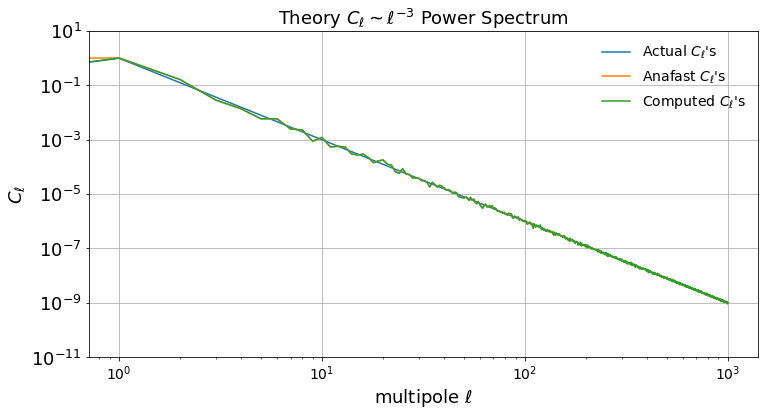
\includegraphics[width=.875\linewidth]{theory_l3_PS.png}}
    \caption{The figure above illustrates the theory $C_{\ell} \sim \ell^{-3}$ Power Spectrum using three different methods of computing the corresponding $C_{\ell}$ values. The actual $C_{\ell}$'s, constructed directly from the $\ell$'s are plotted in blue, HEALPix's \texttt{anafast}-constructed $C_{\ell}$'s are depicted in orange, and the manually-computed $C_{\ell}$'s from \texttt{compute\us cls} can be found in green. From the plot, we can see that the actual and anafast $C_{\ell}$'s directly overlay each other, with the computed $C_{\ell}$'s providing a near direct overlay, with some background noise. This is particularly important since it demonstrates the ability to reconstruct the $C_{\ell}$'s manually, along with the accuracy of the helper functions to sort and compute $a_{\ell m}$'s and $C_{\ell}$'s. This provides useful for the resultant Bispectrum calculations later, as many of these underlying functions are used to compute the Bispectrum. Furthermore, some Bispectrum calculations, such as the Convergence Bispectrum, rely on accurate calculations of the Power Spectrum.}\label{fig:theory_l3_PS}
\end{figure}

\begin{figure}[H]
    \centering
    \tcbox{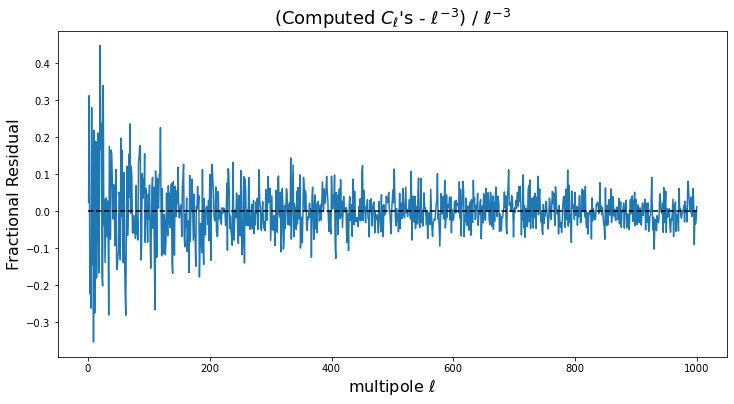
\includegraphics[width=.875\linewidth]{residual_cl.png}}
    \caption{The figure above is a continuation of Fig.~\ref{fig:theory_l3_PS} and shows the fractional residual between the Computed $C_{\ell}$'s from the \texttt{compute\us cls} function against the actual $\ell^{-3}$ field. That is, the noise that was discussed in that figure can be seen here. We can observe that the magnitude of the fractional residual is small, confirming our supposition early that the Computed $C_{\ell}$'s match closely with what they should be, and that the functions used to compute them are accurate for Bispectrum computations later.}\label{fig:residual_cl}
\end{figure}

\begin{figure}[H]
    \centering
    \tcbox{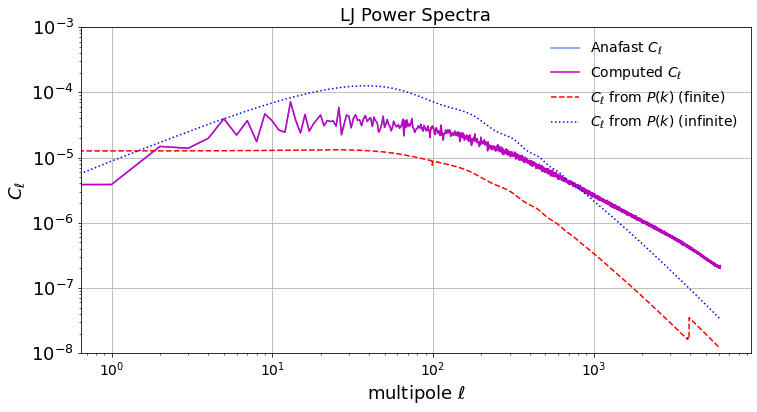
\includegraphics[width=.875\linewidth]{lj_PS.png}}
    \caption{The figure above demonstrates the Last Journey (LJ) Power Spectra using two $C_{\ell}$ computation methods, \texttt{anafast} and manual-computation in solid blue and solid purple respectively, along with $C_{\ell}$ computation from $P(k)$ for the thin finite spherical shell and the infinite shell, in dashed red and dotted blue respectively. More information about Last Journey can be found in \cite{Heitmann_2021}. The first important resultant that we can see from this figure is that, on an actual density map, i.e. the one from Last Journey, the \texttt{anafast} $C_{\ell}$ computation method and the manual computation method of \texttt{compute\us cls} predict the LJ Power Spectrum identically. This confirms the results of Figs.~\ref{fig:theory_l3_PS} and \ref{fig:residual_cl} that the underlying $a_{\ell m}$ sorting and $C_{\ell}$ computation methods work accurately. Then, we can see that the infinite shell computation creates a Power Spectrum of similar shape but different scaling compared to the predicted Power Spectrum, and the thin finite sphrical shell similar but with a different decay around multipole $\ell \sim 10^2$. This overplot is especially important because it culminates the work on the Power Spectra into one final plot, and represents the end for the Power Spectrum phase of the Bispectrum project.}\label{fig:lj_PS}
\end{figure}

\subsection{Bispectrum Plots}\label{bsplots}

The main portion of the Bispectrum, i.e. the Bispectrum calculations and plots, can be divided into three main sections. The first is the initial Last Journey (see \cite{Heitmann_2021} for information about Last Journey) gravitationally-induced weak-lensing Bispectrum plots that were computed from the filter average method of \cite{Munshi_2020}. However, once we went to confirm that the Bispectrum calculations were correct using a theoretical $C_{\ell} \sim \ell^{-3}$ field, as explained in Section~\ref{bispeccalccode}, we found some issues. The second section is devoted to the debugging and fine-tuning of the theoretical Bispectrum calculations on the $C_{\ell} \sim \ell^{-3}$ field. The third section would be devoted to the Convergence Bispectrum, but those plots are still currently being worked on.

\subsubsection{Last Journey Bispectrum}

These figures are the initial gravitationally-induced weak-lensing Bispectrum figures on the Last Journey density map for equilateral $\ell$ triplets (see \cite{Heitmann_2021}). They were computed by taking the even multipole $\ell$ triplets (as the odd ones are just 0) in linear space and in log space. In both figures, i.e. Figs.~\ref{fig:initial_LJ_bispec_linear} and \ref{fig:initial_LJ_bispec_log}, there is a lot of noise in the resultant Bispectrum. These plots were the initial, incorrectly-scaled versions of the Bispectrum computation and using the \texttt{spherical} Wigner-3j function, which, as we know from Section~\ref{wigner}, was prone to errors. These plots are still important to show because they represent the initial test run of the filter average method of computing the Bispectrum from Section~\ref{averagemethod}. Furthermore, they gave an underlying Bispectrum plotting function which I was able to use for testing later. An important note about this is that, since the Bispectrum can have multiple kinds of shapes that are not just the equilateral ones depicted here, such as squeezed and orthogonal, this poses a challenge for plotting | hence why these plots are all for equilateral $\ell$ triplets (in addition to the fact that testing equilateral Bispectrum is more direct).

\begin{figure}[H]
    \centering
    \tcbox{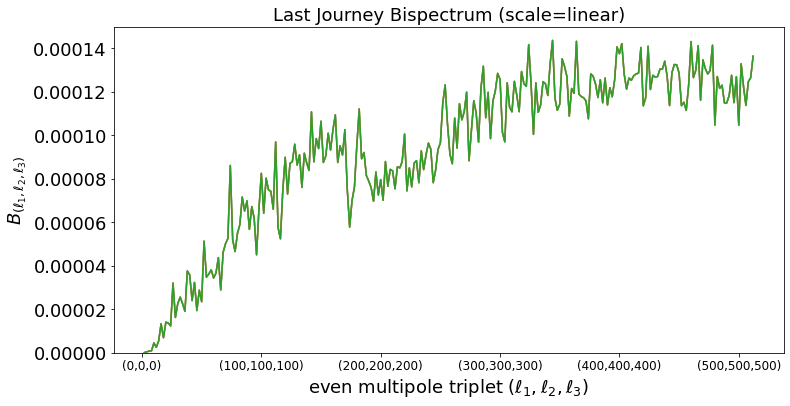
\includegraphics[width=.875\linewidth]{initial_LJ_bispec_linear.png}}
    \caption{The figure above shows the Last Journey Bispectrum plotted on a linear scale for equilateral even $\ell$ triplets. As can be seen, there is a lot of noise in the actual computation.}\label{fig:initial_LJ_bispec_linear}
\end{figure}

\begin{figure}[H]
    \centering
    \tcbox{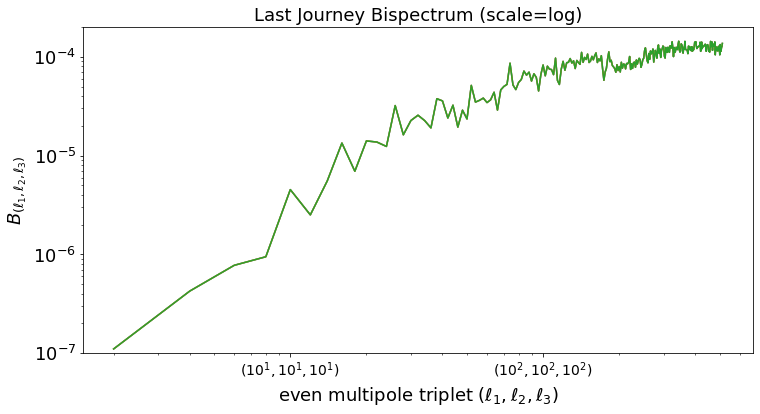
\includegraphics[width=.875\linewidth]{initial_LJ_bispec_log.png}}
    \caption{The figure above shows the Last Journey Bispectrum plotted on a log scale for equilateral even $\ell$ triplets. Similar to Fig.~\ref{fig:initial_LJ_bispec_linear}, there is a lot of noise in the Bispectrum, particularly around multiple triplet $\ell \sim 10^1$.}\label{fig:initial_LJ_bispec_log}
\end{figure}

\subsubsection{Theory Bispectrum Comparison}\label{theorybispecplots}

The figures show key results from when we were testing the filter average method of computing the Bispectrum on a theoretical density field $C_{\ell} \sim \ell^{-3}$. As explained in Section~\ref{bispeccalccode}, during this testing, we discovered some issues in the scaling of the code, and these plots were instrumental in fixing those issues.

\begin{figure}[H]
    \centering
    \tcbox{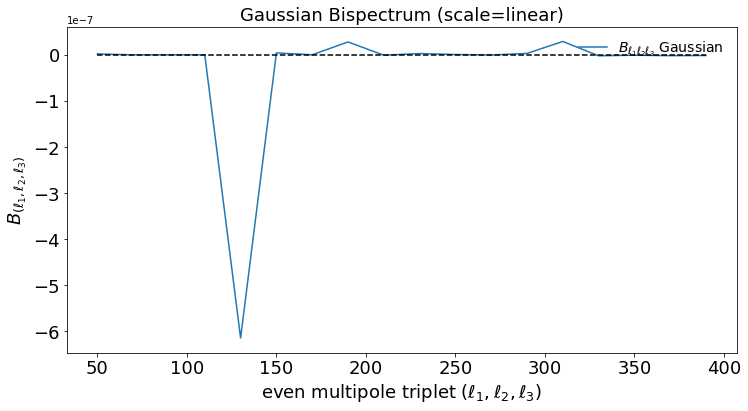
\includegraphics[width=.875\linewidth]{gaussian_bispec_linear.png}}
    \caption{The figure above illustrates the Gaussian gravitationally-induced weak-lensing Bispectrum on a linear scale for equilateral even multiple triplets $(\ell_1, \ell_2, \ell_3)$ using the filter average method and the \texttt{pywigxjpf} Wigner-3j functions. There is one large spike around $\ell \sim 125$, with some other small noise spikes around $\ell \sim 195$ and $\ell \sim 315$. However, these are on the order of $10^{-7}$, indicating that these spikes are likely just background noise. The Bispectrum we computed should theoretically be very close to $0$ because it is Gaussian (and the Bispectrum is a measure of non-Gaussianity, see Section~\ref{intro}), implying that any noise in the resultant computation would be exacerbated when plotting. The Bispectrum computed for a non-Gaussian map, such as Last Journey, we would likely see a lot distribution on an order-of-magnitude a lot higher than $10^{-7}$, trumping the small noise variation we see above. During testing, the scaling of the noise seen above was a lot larger, on the order of $10^{-2}$, indicating that there was a problem with the Gaussian Bispectrum computation. After fixing some missing factors and method-testing our Wigner-3j calculations, as described in Section~\ref{wigner}, we found the key finalized plot above for the theoretical $\ell^{-3}$ field.}\label{fig:gauss_bispec_linear}
\end{figure}

\begin{figure}[H]
    \centering
    \tcbox{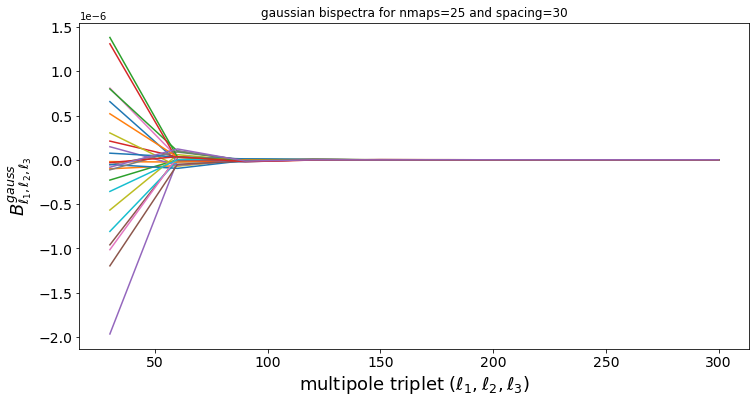
\includegraphics[width=.875\linewidth]{25maps.png}}
    \caption{The figure above highlighs the Gaussian Bispectra as computed for $25$ maps, with intervals of $\ell = 30$ between Gaussian Bispectra computation for $\ell$ triplets in the range of $\ell \in [0,300]$. Each line color represents the Gaussian Bispectra computed for each different map. We can see that there is a lot of spread in the initial computation of the Bispectrum up to around $\ell \sim 60$, but by $\ell \sim 85$, they all seem to even out to around 0. Importantly, the spread is all around a range of $B_{\ell_1 \ell_2 \ell_3} \in [-2.0\cdot 10^{-6}, 1.5 \cdot 10^{-6}]$ | a relatively low order-of-magnitude range. As explained above, since the Gaussian Bispectrum should be close to $0$, the low values of this Bispectrum was a good indicator to us that we are probably just seeing some noise from the $C_{\ell} \sim \ell^{-3}$ field that will be trumped by a Bispectrum computation on an actual non-Gaussian density field. The converging of all of the Gaussian Bispectra of the $25$ maps to 0 after $\ell \sim 85$, is what we would expect, which is also a positive indicator.}\label{fig:25maps}
\end{figure}

\begin{figure}[H]
    \centering
    \tcbox{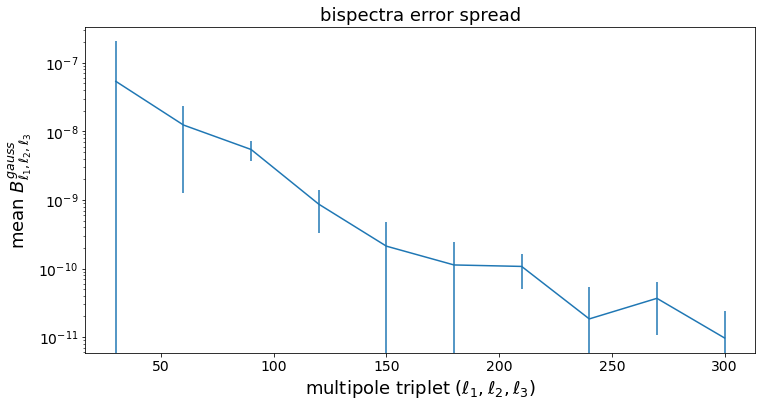
\includegraphics[width=.875\linewidth]{errorspread.png}}
    \caption{The figure above is a continuation of Fig.~\ref{fig:25maps}, as it highlights the error spread of the mean Gaussian bispectra for the maps above. It can be observed from the plot that our error spread is pretty small, on the order of $B^{\rm gauss}_{\ell_1 \ell_2 \ell_3} \sim 10^{-7}$ to  $B^{\rm gauss}_{\ell_1 \ell_2 \ell_3} \sim 10^{-11}$.}\label{fig:errorspread}
\end{figure}

\begin{figure}[H]
    \centering
    \tcbox{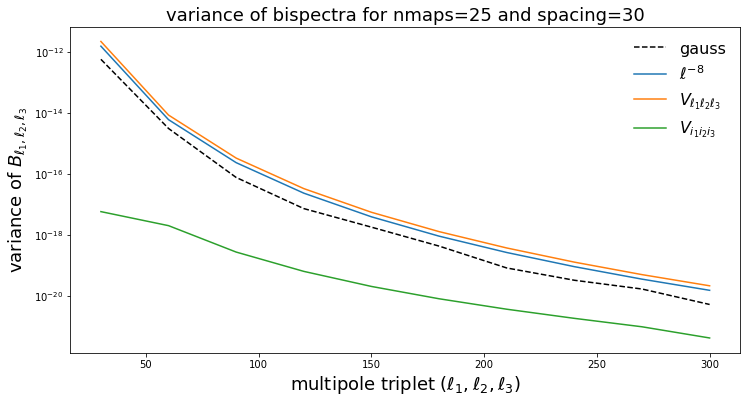
\includegraphics[width=.875\linewidth]{variance.png}}
    \caption{The figure above demonstrates the computed variances for the Gaussian Bispectra of the $25$ maps from Figs.~\ref{fig:25maps} and \ref{fig:errorspread}. The black dashed line represents the Gaussian variance, as computed from \cite{Munshi_2020}. The solid blue line represents the theoretical $\ell^{-8}$ variance of a $C_{\ell} \sim \ell^{-3}$ field. The solid orange line represents the computed $V_{\ell_1 \ell_2 \ell_3}$ variance that is to be expected from the filter average method of Bispectrum calculation, as outlined in Section~\ref{averagemethod}. Finally, the solid green line represents the computed $V_{i_1 i_2 i_3}$ variance that is to be expected from the \textit{binned} Bispectrum estimator for the filter average method of Bispectrum calculation, as also outlined in Section~\ref{averagemethod}. From the plot, we can observe that the predicted variance $V_{\ell_1 \ell_2 \ell_3}$ follows closely with a variance of $\ell^{-8}$ that is expected for the theoretical field we used, and is very close to the Gaussian variance as well. This is important because the reason for using a theoretical field in the first place was to confirm the accuracy of our Bispectrum calculations and resulting variance calculations from \cite{Munshi_2020} against something that we can directly compare it against, i.e. the $C_{\ell} \sim \ell^{-3}$ field. Since all three of these variances follow each other closely, we were able to determine that the Gaussian Bispectrum calculations from \cite{Munshi_2020} were likely computed mostly correctly. The solid green $V_{i_1 i_2 i_3}$ is there for the binned case of the Gaussian Bispectrum as a reference point. Obviously, it does not follow the non-binned estimator case, as expected. A future test would be to go back and plot the variance of our now fully-functioning binned Bispectrum estimator against this expected variance $V_{i_1 i_2 i_3}$.}\label{fig:variance}
\end{figure}

Overall, what we observed from these gravitationally-induced weak-lensing Bispectrum computations on a theoretical field is that we were on the right track, albeit with some scaling issues here and there. The plot infrastructure was also good for testing, and proved extremely useful for the Map method of Bispectrum computation in Section~\ref{mapmethod}. As explained in Section~\ref{bispeccalccode}, once we fixed the scaling issue in the filter average method with the help of the map method code, we were able to finalize a Bispectrum calculator and compile it all into \texttt{bispec\us calculator.py}. Using this updated and hopefully correct gravitationally-induced weak-lensing Bispectrum calculator on the Last Journey density maps would be a good direction for future research.

\subsubsection{Convergence Bispectrum}\label{conv_bispec_plots}

\begin{figure}[H]
    \centering
    \tcbox{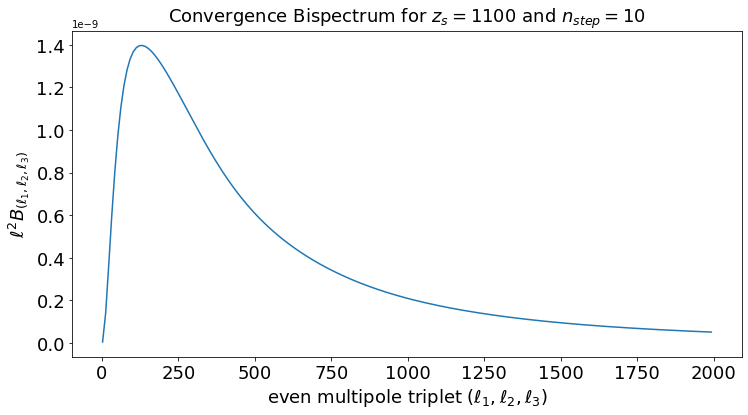
\includegraphics[width=.875\linewidth]{convergence_bispec.png}}
    \caption{The figure above depicts the Convergence Bispectrum for the CMB at redshift $z_s = 1100$ for even equilateral multiple triplets $(\ell_1 \ell_2 \ell_3)$ with $\ell_{max} = 2000$ on a linear scale. The underlying cosmology is based on Planck 2018 parameters. The shape follows a very similar structure to that expected for equilateral Bispectra with these parameters from \cite{Namikawa_2019}, but note that there is still a present scaling issue that is being fixed.}\label{fig:conv_bispec_plot}
\end{figure}

\section{Conclusion}

\subsection{Summary}

Overall, this report summarizes code responsible for computing the gravitationally-induced weak-lensing Bispectrum via two different methods from \cite{Munshi_2020} | namely the filter average method and the map method | along with the Convergence Bispectrum from \cite{Namikawa_2019}. Information about this code, and the Github Repository that houses it, can be found in Section~\ref{code}. This report further compiles much of the theory and supporting papers necessary to create this code in Section~\ref{theory}. Section~\ref{methodology} also includes pertinent information about the methodology and techniques used to calculate the Bispectrum using Numba and Wigner-3j calculators, along with issues that arose during this process, in Sections~\ref{numba} and \ref{wigner}. Relevant figures that were found using this code can be found in Section~\ref{relevant_figures} as they were applied to Last Journey data (see \cite{Heitmann_2021}) and theoretical data. Information about the Bispectrum and the project itself can be found in Section~\ref{intro}. Directions for Future Research in the weak-lensing Bispectrum can be found in the next section (Section~\ref{future_research}). Concluding Thoughts and Acknowledgements can be found in Sections~\ref{finalthoughts} and \ref{acknowledgements} respectively.

\subsection{Directions for Future Research}\label{future_research}

There are four main directions for future research, which I will classify into two short term and two long term tasks.
\npar
The first short term task to work on includes fixing up a few of the scaling issues we had with the convergence bispectrum calculations, which we are currently in the process of doing, and then making sure that they agree with some of our previous plots. There were a few missing $h$ factors and unitary $c$ factors in the initial write-up for the Convergence Bispectrum code that caused the power spectrum $P(k)$ to be slightly off by a few orders of magnitude. Fixing these issues should allow us to find a convergence bispectrum in agreement with previous calculations from \cite{Namikawa_2019}.
\npar
The second short term task would be to confirm and package up the full Bispectrum Calculator, then make sure it works with Argonne HACC simulations. This way, we can test different initial conditions and non-Gaussianities on the Bispectrum calculator and see how they stack up. The first step in doing this would be to actually test the gravitationally-induced weak-lensing Bispectrum calculator in \texttt{bispec\us calculator.py} on a few Last Journey density maps, and possibly again on the theoretical $C_{\ell} \sim \ell^{-3}$ field, to confirm accuracy. Once we confirm this and package things up, then we can move on to integrating with Argonne HACC simulations.
\npar
For the first long term task, looking into the effects of masking would be an important direction for future research. Masking refers to the process of flagging or excluding certain areas of the map where data might be missing or contaminated by foreground sources. These masked regions can introduce complications when calculating statistical measures like the bispectrum. This is important because our maps might not always be of the full sky, either because of contamination or just because we are looking at a smaller portion of the sky Investigation these impacts and how can account for masking would be very important. Two possible methods for doing so that we discussed could include masking-aware estimators and mask inpainting. The former refers to weighing masked pixels differently during bispectrum computation, and the latter refers to filling in the missing or masked regions of the sky maps using interpolation or other statistical methods.
\npar
For the second long term task, since we have a binned version of the bispectrum estimator working, a direction we could take is to look into extending the theory for the weak lensing bispectrum into a binned version and seeing how it differs.

\subsection{Final Thoughts}\label{finalthoughts}

Overall, this project was an exciting and engaging way to learn more about Cosmology and Scientific Computing. I learned a lot about the Power Spectrum, Bispectrum, the CMB, Python, High-Performance Computing, and Computational Cosmology overall, for which I am very grateful and eager to apply in the future. While daunting at times, I am grateful for the opportunity to explore my love of the cosmos through the Bispectrum and Computational Cosmology. This project has a lot more that can be explored, and I can't wait to see where it goes.

\subsection{Acknowledgements}\label{acknowledgements}

Thank you to Dr. Patricia Larsen for being my mentor and guiding me through this Bispectrum project | whose time, dedication, and thoughtfulness was instrumental, and without whom this work would not be where it is today. Thank you to Dr. Salman Habib for giving me this opportunity at Argonne to work on this project and helped me fix the Wigner-3j issues. Thank you to Dr. Michael Buehlmann and Dr. JD Emberson for helping me understand and implement parallelization techniques within my code, and for helping me better understand the Power Spectrum and Bispectrum. A very big thank you to Aurora Cossairt, who always took the time to help me understanding the intricacies of the Power Spectrum and the Bispectrum and the computations behind them. Thank you to Humza Qureshi, who helped advance my Python knowledge as I began working on this project.

\section{Bibliography}

\bibliography{references}

}
\end{document}